%------------------------------------------------------------------------
\begin{frame}{يادآوری}
	\begin{itemize}\itemr
		\item[-]
کتاب CLRS که مرجع اصلی این درس است دو تعریف مجزا برای گراف ارائه می‌دهد:
\item[۱]
گراف بدون جهت: این گراف نمی‌تواند طوقه یا یال موازی داشته باشد.
\item[۲]
گراف جهت دار: این گراف می‌تواند طوقه داشته باشد اما نمی‌تواند یال موازی داشته باشد. البته دو یال می‌تواند بین دو راس یکسان وجود داشته باشد به شرطی جهت آنها مخالف یکدیگر باشد. برای مثال شکل زیر یک گراف فاقد یال موازی است. به این یال‌ها پادموازی
\fn{1}{antiparallel}
 گفته می‌شود.

\begin{figure}[h!]
\centering
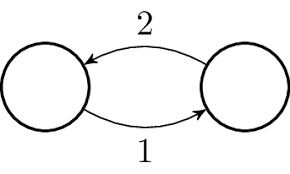
\includegraphics[width=0.2\textwidth]{figs/chap01/1.png}
\end{figure}
\item[-]
در هر یک از مسائل بسته به ذات مسئله نوع خاصی از گراف به عنوان ورودی در نظر گرفته می‌شود. برای مثال ورودی مسئله کوتاه ترین مسیر در حالت کلی یک گراف جهت دار و وزن دار است.
\end{itemize}
\end{frame}


%------------------------------------------------------------------------
\begin{frame}{يادآوری}
	\begin{itemize}\itemr
\item[-]
الگوریتم‌های گراف برخلاف بیشتر الگوریتم‌هایدارای دو متغییر تاثیر گذار در اندازه ورودی‌اند: تعداد یال‌ها (|E|) و تعداد رئوس (|V|) .
\item[-]
بر اساس قرارداد کتاب CLRS می‌توان در نمادهای مجانبی از قرار دادن نماد اندازه در اطراف V و E صرف‌نظر ‌کرد.

\item[-]
الگوریتم‌های گراف به طور معمول در دو حالت بررسی می‌شوند:
\item[الف]
زمانی که گراف متراکم باشد: در این حالت فرض میکنیم همه رئوس به هم متصل هستند بنابراین تعداد یال ها از مرتبه
\ath{V^2}
است.
\item[ب]
زمانی که گراف خلوت باشد:‌ در این حالت به طور معمول فرض می‌شود که تعداد یال‌ها از مرتبه
\ath{V}
است.

	\end{itemize}
\end{frame}

%------------------------------------------------------------------------
\begin{frame}{يادآوری}
\begin{itemize}\itemr
\item[-]
پیچیدگی زمانی ارائه شده برای یک الگوریتم گراف را می‌توان در دو حالت بالا تحلیل کرد. برای مثال تمرین زیر از کتاب CLRS را در نظر بگیرید:

\begin{figure}[h!]
\centering
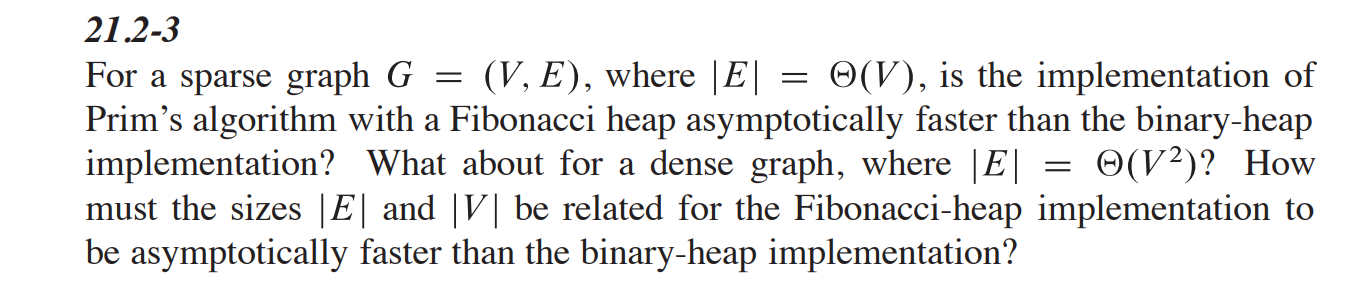
\includegraphics[width=\textwidth]{figs/chap01/2.png}
\end{figure}

\end{itemize}
\end{frame}

%------------------------------------------------------------------------
\begin{frame}{يادآوری}
\begin{itemize}\itemr
\item[-]
پیچیدگی زمانی الگوریتم پریم با استفاده از هرم دودویی از مرتبه
\m{O(E logV+V lgV)}
و با استفاده از هرم فیبوناچی از مرتبه
\m{O(E+V logV)}
است. با جایگذاری V به جای E در این دو تابع درمی‌یابیم که در گراف خلوت هر دو پیاده‌سازی‌ از لحاظ مجانبی سرعت یکسانی دارند و از مرتبه
\m{O(Vlg V)}
اند. اما در گراف متراکم پیاده‌سازی با هرم فیبوناچی از لحاظ مجانبی سریع تر و از مرتبه
\m{O(lgV^2)}
 است.
\item[-]
چنین تحلیلی در دیگر الگوریتم‌‌های گراف هم کاربرد دارد. برای مثال الگوریتم فلوید-وارشال از مرتبه زمانی
\m{O(V^3)}
 است. از تحلیل این تابع می‌توان نتیجه گرفت خلوت یا متراکم بودن گراف از نظر مجانبی تاثیری بر سرعت این الگوریتم ندارد.
\end{itemize}
\end{frame}



